\unfinished{write results}
% Notes: 

% -----------

% What to include:
% Time - Suboptimal extention of sklearn
% Amount of deviation
% Different metrics at different models 
% could run more than 50 but need to run in realistic time on workstation

This section will present and interpret the results from the conducted experiments. There are many experimental setups. Three different models evaluated on five datasets with varying amount of compression. Then in addition to that, there is many metrics to be looked at. To illustrate this comprehensive amount of results, Table \ref{tab:comparison} has been constructed. The Table contains the results of three of the five datasets. The Table will be reffered to repeatedly in the following examination of the results. The values that are reffered to is marked with bold.

\subsection{Execution time}
Starting off with looking at the execution time. The training and test time on the synthetic dataset can visually be seen on Figure \ref{fig:performance_time}. It shows no apparent difference between neither the training time or testing of the original and bases model. However, there is a clear difference between those two and DupRes. Both the training in which the uniques are found and in the testing in which the duplicates are looked up adds additional execution time. This performance cost can also clearly be seen in the table for the pendigits dataset. Here we have 93.7/55.3 ms train/test time for the original model, while DupRes with 1 deviation bit has 135/282 ms train/test time. Additionally, it can be seen that DupRes with 6 deviation bits has 145/131 train/test time. This implies that, as the amount of deviation bits rise the testing time decreases. This makes sense as less uniques are found during the training phase, and thus less entries in the table need to be looked through during testing. This incentivize to not use the model if a low amount of duplicates is expected in the data or a low amount of deviation bits is utilized. Originally an implementation utilizing pandas'\cite{pandas} dataframes was used. However, this performed notably worse then the current implementation which uses numpy\cite{numpy} arrays. To optimize this further an implementation could be made in c or c++ and utilize the interoperability to Python.

\subsection{Metrics and Scoring}
Then we look at the performance of the models in terms of metrics and scoring. Figure \ref{fig:performance_metrics} illustrates the performance metrics of the models on the datasets. Investigating the metrics for the synthetic dataset a clear pattern can be seen

\subsection{Compression and Memory}

\begin{figure}
  \centering
  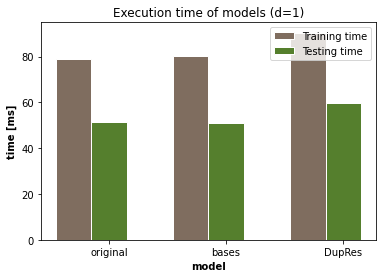
\includegraphics[width=0.8\linewidth]{images/performance_time.png}
  \caption{}
  \label{fig:performance_time}
\end{figure}

\begin{figure}
  \centering
  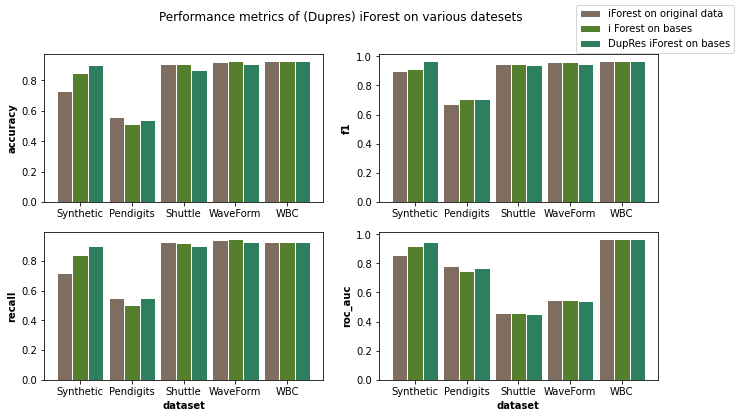
\includegraphics[width=\linewidth]{images/performance_metrics.png}
  \caption{}
  \label{fig:performance_metrics}
\end{figure}



\begin{table*}[t]
  \centering\sffamily
  \renewcommand{\theadfont}{\normalsize\bfseries}
  \setcellgapes{1ex}\makegapedcells
  \begin{tabular}{*{10}{|c}|c|}
    \hline
    \multirowthead{2}{Model} & \multirowthead{2}{Dataset} & \multirowthead{2}{Dev. bits} & \multicolumn{4}{c|}{\bfseries Metric} & \multicolumn{2}{c|}{\bfseries Time} & \multirowthead{2}{Compression Rate} & \multirowthead{2}{Memory Accessed}                                                                   \\
    \cline{4-9}
                             &                            &                              & \textbf{acc.}                         & \textbf{f1}                         & \textbf{rec.}                       & \textbf{roc}                       & \textbf{T(ms)} & \textbf{E(ms)} &                               \\
    \hline
    Original                 & Synthetic                  &                              & 0.73                                  & 0.84                                & 0.72                                & 0.86                               & 78.8           & 51.4           & 0\%    & 100\%                \\

    \cline{2-11}
                             & Pendigits                  &                              & 0.54                                  & 0.70                                & 0.54                                & 0.77                               & \textbf{93.7}  & \textbf{55.3}  & 0\%    & 100\%                \\

    \cline{2-11}
                             & WBC                        &                              & 0.94                                  & 0.97                                & 0.94                                & 0.97                               & 75.2           & 22.0           & 0\%    & 100\%                \\
    \hline

    \multirow{9}{*}{Bases}   & \multirow{3}{*}{Synthetic} & 1                            & 0.72                                  & 0.83                                & 0.71                                & 0.86                               & 80.2           & 51.2           & 12.5\% & 87.5\%               \\
    \cline{3-11}
                             &                            & 3                            & 0.90                                  & 0.95                                & 0.90                                & 0.95                               & 74.6           & 46.4           & 37.5\% & 62.5\%               \\
    \cline{3-11}
                             &                            & 6                            & 0.04                                  & 0.00                                & 0.00                                & 0.5                                & 74.3           & 45.0           & 75.0\% & 25.0\%               \\
    \cline{2-11}
                             & \multirow{3}{*}{Pendigits} & 1                            & 0.53                                  & 0.70                                & 0.53                                & 0.77                               & 95.1           & 55.7           & 12.5\% & 87.5\%               \\
    \cline{3-11}
                             &                            & 3                            & 0.51                                  & 0.67                                & 0.51                                & 0.75                               & 94.3           & 55.9           & 37.5\% & 62.5\%               \\
    \cline{3-11}
                             &                            & 6                            & 0.42                                  & 0.59                                & 0.41                                & 0.68                               & 95.3           & 56.0           & 75.0\% & 25.0\%               \\
    \cline{2-11}
                             & \multirow{3}{*}{WBC}       & 1                            & 0.94                                  & 0.97                                & 0.94                                & 0.97                               & 75.3           & 21.6           & 12.5\% & 87.5\%               \\
    \cline{3-11}
                             &                            & 3                            & 0.94                                  & 0.97                                & 0.94                                & 0.97                               & 75.6           & 21.6           & 37.5\% & 62.5\%               \\
    \cline{3-11}
                             &                            & 6                            & 0.95                                  & 0.97                                & 0.94                                & 0.97                               & 74.8           & 21.4           & 75.0\% & 25.0\%               \\
    \hline
    \multirow{9}{*}{DupRes}  & \multirow{3}{*}{Synthetic} & 1                            & 0.87                                  & 0.93                                & 0.86                                & 0.93                               & 90.4           & 59.7           & 12.5\% & 87.5\% + count table \\
    \cline{3-11}
                             &                            & 3                            & 0.92                                  & 0.95                                & 0.91                                & 0.96                               & 85.8           & 55.4           & 37.5\% & 62.5\% + count table \\
    \cline{3-11}
                             &                            & 6                            & 0.98                                  & 0.99                                & 1.00                                & 0.75                               & 86.5           & 53.4           & 75.0\% & 25.0\% + count table \\
    \cline{2-11}
                             & \multirow{3}{*}{Pendigits} & 1                            & 0.54                                  & 0.70                                & 0.53                                & 0.76                               & \textbf{135}   & \textbf{282}   & 12.5\% & 87.5\% + count table \\
    \cline{3-11}
                             &                            & 3                            & 0.50                                  & 0.67                                & 0.50                                & 0.75                               & 135            & 286            & 37.5\% & 62.5\% + count table \\
    \cline{3-11}
                             &                            & 6                            & 0.80                                  & 0.89                                & 0.80                                & 0.77                               & \textbf{145}   & \textbf{131}   & 75.0\% & 25.0\% + count table \\
    \cline{2-11}
                             & \multirow{3}{*}{WBC}       & 1                            & 0.94                                  & 0.97                                & 0.94                                & 0.97                               & 86.9           & 23.4           & 12.5\% & 87.5\% + count table \\
    \cline{3-11}
                             &                            & 3                            & 0.94                                  & 0.97                                & 0.94                                & 0.97                               & 87.7           & 23.7           & 37.5\% & 62.5\% + count table \\
    \cline{3-11}
                             &                            & 6                            & 0.95                                  & 0.97                                & 0.94                                & 0.97                               & 85.6           & 23.5           & 75.0\% & 25.0\% + count table \\
    \hline
  \end{tabular}
  \caption{Table of stuff}
  \label{tab:comparison}
\end{table*}